\documentclass{article}
\usepackage[english]{babel}
\usepackage[utf8]{inputenc}
\usepackage[explicit]{titlesec}
\usepackage[margin=1.5in]{geometry}
\usepackage{graphicx}
\usepackage{tabularx}
\usepackage[none]{hyphenat}
\usepackage{enumitem}
\usepackage{titlesec}
\usepackage[bookmarks]{hyperref}

\newcommand{\sectionbreak}{\clearpage}

\addtolength{\parskip}{-0.5mm}
\setlength{\parskip}{1em}
\setcounter{secnumdepth}{4}

\newcommand{\myparagraph}[1]{\paragraph{#1}\mbox{}\\ \newline}

\begin{document}
\noindent
This document is incomplete and not intended for public consumption. Some grammatical errors and language inconsistencies have not yet been corrected. Some citations are missing. Aspects are subject to change.

\pagebreak

\title{{\bfseries Block Sports}: A decentralized sports betting exchange}
\renewcommand{\arraystretch}{1}
\author{
	\footnotesize
	\hspace*{+.4cm}
	\begin{tabularx}{\textwidth}{ p{3.75cm} p{3.75cm} p{3.75cm}}
		\begin{center}
		\item {\bfseries Mirren King-Smith} \texttt{mirren@blocksports.com} 
	 	\end{center} &
	 	\begin{center}
		\item {\bfseries Tsering Redmond} \texttt{tsering@blocksports.com}
	 	\end{center} &
	 	\begin{center}
		\item {\bfseries Sergej Stojanovski} \texttt{sergej@blocksports.com}
	 	\end{center}
	\end{tabularx}
}

\date{}

\maketitle
\renewcommand{\arraystretch}{2}

\begin{abstract}

\setlength{\parskip}{1em}

There has been a recent rise in cryptocurrency based betting services to meet the demand of a market that prefers its use over fiat currency. While popular, these escrow services follow an unfavorable trend of utilizing cryptocurrency in a centralized manner, creating counterparty risk that did not previously exist. This occurs as users entrust the ownership of their cryptocurrency to services which are susceptible to hacks and leave little recourse to victims of theft. We propose a sports betting exchange which solves this issue by means of decentralization, removing central points of failure to allow the use of cryptocurrency without counterparty risk. 

A sports betting exchange is a marketplace for the trade of sporting outcomes. Unlike a traditional sports betting platform, a sports betting exchange eliminates the need for a central bookkeeper and instead enables users to place bets against one another. This paper details Block Sports, a decentralized sports betting exchange that approaches the concept of a blockchain-native sports betting platform with two key objectives --- creating a decentralized and trusted framework for sports betting and providing a rich user experience through an off-chain service layer. Utilizing the Neo blockchain, a solution is proposed which integrates a decentralized oracle consensus network with a series of smart contracts, allowing users to place bets on sporting outcomes with NeoGas (GAS). The result is a platform that solves the issue of counterparty risk while still remaining competitive with traditional sports betting exchanges.

\end{abstract}

\pagebreak

\section{Introduction}

Cryptocurrency was developed as an electronic cash system that could operate without the oversight of financial institutions. By removing the need for centralized governance a trustless form of payment was created, eliminating third-party interference and giving users true ownership over their funds. Cryptocurrency has proven itself as a successful alternative to fiat currency, with an increasing number of individuals preferring it is as a form of payment for products and services.
 
Although this new form of currency is perfect for direct exchange, issues arise with its use in centralized escrow services such as currency exchanges and betting platforms. These services introduce a new kind of counterparty risk as users are required to forgo the ownership of their cryptocurrency by putting their trust in the hands of service operators. In a traditional, fiat-based service this risk is counteracted by the governance of financial institutions. However when cryptocurrency is used in centralized escrow services there are limited recourse options for the victims of loss and theft.

Despite a significant focus on security, centralized escrow services such as currency exchanges have fallen prey to a number of major hacks and thefts, costing users hundreds of millions in USD equivalent. Most notably the theft of Mt. Gox, Bitfinex and more recently BitGrail demonstrate that even the most trusted services are inherently insecure. As a consequence of these hacks there has been a demand for decentralized escrow services which can operate without the requirement of a central authority. If the service operator has no administrative control little is gained from compromising the service. While there has been a rise in decentralized currency exchanges to combat this issue, no adequate solution has been developed to protect cryptocurrency betting services. 

This paper details Block Sports, a sports betting exchange which provides a solution to the counterparty risk found in cryptocurrency based betting platforms. This solution is achieved through the decentralization of its critical architecture, removing administrative control over functionality which may impact user’s funds. Using the Neo blockchain a proposal is put forward for a decentralized, peer to peer sports betting platform.

	\subsection{Why Neo}
Several blockchain platforms were considered for the Block Sports Exchange, our conclusion was that Neo is most suitable for the following reasons.

		\subsubsection{Blockchain Performance}
Speed and transaction volume are perhaps the most important aspects needed in a blockchain to support the adoption of mass market applications. Slow and congested platforms do not lend themselves to a great user experience, especially for applications such as sports betting exchanges which see constant updates and high transaction volume. Poor performance can severely hamstring liquidity and volume which are crucial to a sports betting exchanges success. In the case of scalability and performance the Neo blockchain holds a leading position due to a byzantine fault-tolerant consensus mechanism, with the theoretical capacity to perform thousands of transactions per second.

		\subsubsection{NEO Generates GAS}
NeoGas (GAS) will be the sole utility token used for betting on the Block Sports Exchange. Any person who owns NEO is generating GAS, therefore any person holding NEO will be ready to use the Block Sports Exchange from day one. This greatly increases the potential user base of Block Sports. Furthermore using GAS as the platform currency will significantly increase liquidity and reduce volatility than instead forcing the use of a native utility token with a much smaller market capitalization.

		\subsubsection{Language Accessibility}
Smart contract enabled platforms generally have singular language support, sometimes utilizing their own custom language as the only choice. Neo’s support for multiple languages improves development accessibility, making it easier to help transition new employees into developing for the Neo blockchain.

	\subsection{Why Sports Betting}
A decentralized sports betting exchange is at the perfect intersection of three market factors - use case, existing market and competition. 

		\subsubsection{Use Case}
The cryptocurrency ecosystem has been rife with products that shoehorn decentralized technology into areas which do not necessarily benefit from the inclusion. While this experimentation is expected, companies without distinct market value or monetization methods bring into question their longevity as a product and value as an investment. A sports betting exchange not only has a clear monetization system, it has a clear use case --- providing sports betting to holders of cryptocurrency.

		
		\subsubsection{Existing Market}
Over 150 billion USD is bet on sports betting per year in the United States alone, accounting for almost 1\% of the GDP. World wide, it is estimated that 900 billion USD is placed on sports betting per year. Although there are no exact statistic for the overlap of individuals who use cryptocurrency and bet regularly, the size of both the betting and cryptocurrency markets create the safe assumption of a large existing user base. Regardless of this intersection, the end goal for Block Sports is to provide enough value from a security and usability standpoint that we can begin to target the mainstream betting audience with our platform. 

		\subsubsection{Competition}
There are currently no existing solutions in market which provide a decentralized sports betting exchange. While there are projects announced which target this same area, we believe our solution will have better performance due to the Neo blockchain and greater decentralization due to the oracle consensus network.

\pagebreak

\section{Background}

	\subsection{Sports Betting Exchange}
A sports betting exchange is a marketplace for bettors to trade on the outcome of sporting events. As opposed to a traditional sports betting platform, a sports betting exchange allows bettors to bet against each other, rather than against ‘the house’. Similar to a currency exchange where the market forces of bids and offers determine the price of a currency, the market forces of back and lay betting in a sports betting exchange determine the odds for an outcome.

		\subsubsection{Backing and Laying}
Traditional sports betting platforms restrict users to backing the outcome of an event (betting on the outcome happening). A sports betting exchange takes this concept further and enables users to bet on both the outcome happening and not-happening. This is referred to as ‘backing’ (betting for an outcome) and ‘laying’ (betting against an outcome). 

The ability to back and lay is what allows users to trade the outcome of events. This simply means that if a ‘back’ bet is placed on an outcome, that outcome must happen for the user to win, if anything else happens the counter ‘lay’ bet wins.

				\myparagraph{Backing Example}
\medskip 
The calculation of a back bet is simply:  

\begin{equation}
P = S\times(O - 1)\label{eq:backing}
\end{equation}

Using Equation \ref{eq:backing}, a back bet with the odds of 4 and a stake of 0.5 GAS would generate 1.5 GAS profit:

\begin{equation}
1.5 = 0.5\times(4 - 1)\
\end{equation}

Where P is profit (total return - initial stake), S is the bettor's stake and O is the given odds.

				\myparagraph{Laying Example}
\medskip
Equation \ref{eq:backing} can be updated slightly to indicate the liability required to cover a bettor's stake: 

\begin{equation}
L = S\times(O - 1)\label{eq:laying}
\end{equation}

Where L is liability, S is the bettor's stake and O is the given odds.

Using Equation \ref{eq:laying}, a lay bet to cover a 6 GAS stake with odds of 2.5 would require a 9 GAS liability:

\begin{equation}
9 = 6\times(2.5- 1)\
\end{equation}

In this example the lay bettor would receive a 6 GAS profit if the outcome favoured them.

			\subsubsection{Betting Exchange vs Bookmaker}
Although betting exchanges can be more challenging to navigate for some users due to their increased complexity, they have proven quite disruptive to traditional betting platforms operated by bookmakers as they are superior for several reasons. 

				\myparagraph{Best Odds Possible}
Traditional bookmakers set their own odds with a hefty margin included, whereas betting exchange odds are better than their counterpart as they are determined by the users of the platform. In a space where a 1\% edge over time is the difference between success and failure, having the best odds available is the most important distinction for serious bettors. 

				\myparagraph{Arbitrage}	
Odds on a betting exchange are dynamic and constantly changing, providing opportunity for arbitrage for bettors to capitalise on the variant odds across marketplaces. This is most commonly achieved by trading bots utilising exchange APIs.

				\myparagraph{Back Out of Bets}		
Due to the ability to back and lay, users are able to ‘back out’ of a bet by simply placing an equal valued bet on the opposing outcome, in turn hedging their existing bet. Similar to a currency exchange where users can scalp trades when prices change, this mechanism allows users to scalp bets as odds change.

			\subsubsection{Centralized vs Decentralized Betting Platforms}
In the case of a decentralized sports betting platform vs a centralized platform there is a clear difference from a user perspective. A centralized platform benefits from efficiency and performance that can not be rivaled by the slower performance of a blockchain operated platform. However we can argue that the performance of a decentralized betting exchange is more than adequate for most user needs and that this advantage is far less integral than those of a decentralized platform.

				\myparagraph{Account Control}					
Bans, denial of service and increased fees are not uncommon occurrences for users on centralized platforms. Ultimately the platform operator has control of user access where at any time they can deem a user on the platform undesirable. This is often only due to a user winning too much or having too high a volume. Censorship resistance is an inherent advantage of decentralized platforms and cryptocurrency. This advantage extends to decentralized betting platforms as the operator has no ability enforce discrimination over specific users.

				\myparagraph{Withdrawal Fees and Limitations}			
Withdrawals on centralized fiat betting platforms can take hours or days to process and often have significant fees attached due the necessity of third parties such banks and payment gateways. Although deposit and withdrawal to a smart contract is still necessary on a decentralized betting platform, no third party verification is required apart from that of blockchain consensus, resulting in relatively fast transaction speeds and low or no fees. Furthermore it is common for centralized fiat platforms to lock user funds until certain verification or assessment is complete which is not the case for decentralized betting platforms. 

				\myparagraph{Security}		
The most important advantage of a decentralized betting platform is security of funds and integrity of data. There is no shortage of centralized sports betting platforms that utilize cryptocurrency, however users are required hold their cryptocurrency in escrow on these platforms, abandoning their ownership. As previously mentioned this creates counterparty risk and has led to situations where funds have been lost or stolen by centralized escrow services.		
	
	\clearpage
	\subsection{Achieving Decentralization}
In the context of platform decentralization it is important to define exactly what decentralization means. We argue that there are two primary aspects of a decentralized platform, security and autonomy. However many platforms that are considered decentralized may be secure but not completely autonomous. For example Switcheo, a decentralized exchange on the Neo blockchain, is far more secure than a centralized exchange due to the utilization of smart contract processing but is not completely autonomous. This is due to aspects of the exchange such as the front end application being reliant on its platform operators for hosting. If the front end service layer became unavailable the exchange would not be accessible to users. What makes the platform decentralized is that this would not be considered a critical failure as funds would still be secured on-chain and accessible by other means. 

For the Block Sports Exchange, the level of decentralization will be similar to that of Switcheo and many other decentralized platforms. Operating all integral aspects of the platform on-chain ensures security while some non-critical aspects such as a front end service layer and a public API will still be controlled and operated by the Block Sports team. If any of these non-critical aspects were hijacked and used for nefarious means, the risk would be low as verification would still be an on-chain process [see section x]. Granted this solution is not completely autonomous however is an adequate solution to the core problem of counterparty risk set out in the introduction. 

Block Sports Exchange requirements for decentralization:
\begin{itemize}
	\item All escrow and processing of funds handed on-chain
	\item Matching verification handled on-chain
	\item Match and outcome data reporting must be distributed among multiple parties and reach consensus
	\item Core exchange functionality can be performed without any centralized governance through direct invocation  
\end{itemize}

It should be noted that a critical aspect of the platform, the oracle network will not initially be autonomous as it will be operated by the Block Sports team. This will be eventually transitioned to complete autonomy [see section 6 for details]. 
		
\section{Platform Overview}

	\subsection{Anonymity}
Anonymity has a large part to play in the empowerment of cryptocurrency users. Introducing mandatory preconditions to access the Block Sports platform, such as the verification of personal details, removes anonymity and defies the core objectives of Block Sports and cryptocurrency in general. The freedom provided by the blockchain to maintain anonymity is preserved on the Block Sports exchange by allowing the user to place and retrieve bets without the need for a user account. The only prerequisite for betting is the existence of a wallet containing NeoGas (GAS). 

User accounts are an optional feature on the Block Sports exchange, requiring no personal information. Accounts are instead used for notifications, history tracking and personalized account preferences, tied to a login which users can access throughout multiple sessions.

	\subsection{Oracle Network}	
The operation of a sports betting exchange is dependent on real world data sources to provide event details such as fixtures and outcomes. In a centralized scenario a single authority is trusted to report this event information to the platform. If we consider the failure of this authority to report correct information we realize this leads to the improper loss of user funds and a reduced trust in the platform. Given that users are unable to turn to governing authorities for recourse in the case of loss, placing funds on the platform is a risk users may not want to take. Therefore it is important that Block Sports puts measures in place to eliminate the danger of incorrect reporting.

To solve this problem, a solution is proposed by utilizing multiple independent networked oracle nodes. These oracles are community run programs responsible for publishing event data to the blockchain, only finalizing data that has achieved a majority consensus across these nodes. By removing the responsibility from a single entity and distributing it across trusted owners, a trusted consensus mechanism for event data is possible [see section 6 for detailed information]. To incentivize community members to help operate an oracle, all operators are entitled to a direct share in fees collected from the Block Sports exchange. [see section 8 for more detail].

	\subsection{Exchange API}
Similar to currency and commodity exchanges a significant portion of volume on sports betting exchanges is traded by bots via an exchange API. For most professional bettors with significant capital an exchange API is an essential feature as it enables calculated trading much faster than any manual trading via the exchange interface. Volume is one of the most important factors for a successful betting exchange, hence API access is fundamental to maximising volume on the Block Sports Exchange.	

	\subsection{User Experience}
A seamless user experience is essential to the larger commercial success of the Block Sports Exchange. A decentralized application which can appear separate from the blockchain while maintaining decentralization is an ideal solution in a space where applications often cripple user experience with poor design and confusing workflows. It is important that users familiar with centralized sports betting exchanges do not feel that the user experience on the Block Sport Exchange is diminished by the constraints of decentralization. 

It is the intention of Block Sports to remain competitive with existing sports betting exchanges by providing all features that users familiar with leading sports betting exchanges would be accustomed to.

	\subsection{Private Bets}
Private betting enables users to place bets amongst themselves in a secure and trustworthy setting, allowing them to formalise bets on the Neo blockchain. As an example, this feature could be used by friends watching a sporting match in person or users on a forum that wish to formalise a bet with a trusted arbiter at odds they agree upon personally. Given that an exchange framework will exist for creating and resolving bets, the addition of private betting can be recognized as a natural extension of architecture.

	\subsection{Medium of Exchange}
As the Block Sports exchange is a decentralized platform, cryptocurrency is required as the medium of exchange. The solution implemented by other platforms involves the creation of a new, native utility token to act as the platform currency. Although there are regulatory advantages to creating a utility token as opposed to a security token, this solution present several drawbacks and is in fact detrimental for both users and investors. A far better solution which also benefits the Neo ecosystem is the utilization of a pre-existing utility token, NeoGas (GAS). Using GAS as the platform currency significantly increases liquidity and reduces volatility compared to requiring the use of a native utility token with a much smaller market capitalization. Furthermore, utilizing GAS allows the function of the Block Sports token (BSX) to have more benefits than other utility tokens whose only value is their required use on their platform [see section 8 for more on BSX token].

	\subsection{Limitations}
The use of blockchain technology as a platform foundation does not come without its limitations. While there are many benefits, there are also functional constraints which may impact users accustomed to traditional sports betting exchanges. Although it is important to understand the limitations, we do not believe these will significantly impact the commercial success of Block Sports.  

		\subsubsection{Block Times}
Updates are not published to the blockchain until a new block has been generated. The time taken to perform consensus and publish a new block is referred to as the block time. In the case of the Neo blockchain the block time is typically between 15 to 30 seconds. During this period updates are delayed until all information such as transactions and invocations received are processed and verified. As a result, users may have to wait up to a full block time for their bets, cancellations and withdrawals to be performed. For the average user this is not an issue and will only present itself as an inconvenient delay. However, for some professional bettors this may affect their ability to arbitrage bets in certain scenarios.

		\subsubsection{In-Play Betting}
In-play betting is the ability to place bets during a live event. This feature is typically only offered on popular events and accounts for a minority of sports betting volume. While implementing in-play betting on the Block Sports Exchange is technically possible, enabling this may lead to situations that are unacceptable to users.
 
One such situation is the requirement for consensus and publication of event results by oracles. While an event may have already concluded it would be required for the oracle to update this event before bets could be suspended. This delay would allow users to place bets on a known outcome before they can be disabled.
 
In a similar scenario, if a play is made which is perceived as outcome altering there will exist an unfair opportunity to place bets before market reaction. Even with instantaneous transactions, traditional exchanges are susceptible to users capitalizing on this vulnerability by means of ‘ring-side betting’, therefore adding block time delays will only work to compound this issue. 

As a result of this, live betting will not be available on the Block Sports Exchange until a satisfactory solution is established either by improved block times or an alternate solution is conceived. 

		\subsubsection{Immutable Outcomes}
Although immutability is an integral aspect of a blockchain it can be problematic in some scenarios. In the highly rare case that consensus is met on a data source that reported incorrect information - for example an outcome was misreported or a ruling was later overturned - the result of the bet can not be reversed. In the case of a centralized exchange, there is typically a short withdrawal delay on user funds in case any misreporting occurs allowing funds to be returned to the correct winners. However this delay imposed by centralized exchanges only accounts for some of the misreported outcomes that happen shortly after the initial outcome was reported. After this delay it is uncommon for a service to compensate lost funds as liability is placed on the user. As there is no verification delay imposed on Block Sports Exchange withdrawals, funds are accessible immediately after an outcome consensus is met. If this situation occurs users affected will be liable for any loss as result of a misreport. In the event of this rare case, Block Sports may decide to compensate users however this will at the discretion of management.

		\subsubsection{Betting Markets}
For initial release, Block Sports is focused on solely providing head to head sports markets. This is less a technical limitation and more a design decision, reducing developmental complexity in order to release the product to market sooner. By reducing the number of markets we also reduce the spread of liquidity across the platform during the early stages of its growth.

\section{Architecture Overview}
The Block Sports Exchange relies on the union of two separate systems to operate. Firstly, a decentralized exchange infrastructure built on the NEO blockchain and secondly, a centralized  off-chain service layer. Making this distinction brings attention to the objectives of both systems, where the exchange layer aims to enable critical functionality through decentralization and the off-chain service layer exists to make user interface to this infrastructure as accessible as possible.  

Figure \ref{figure:architecture} provides an overview of the platform infrastructure and illustrates a high level platform workflow. To break down each stage:
\begin{enumerate}[label=(\alph*)]
	\item Third party data sources which provide oracles with event information
	\item Off-chain oracle network which draws from third party sources and works to publish event information to the blockchain 
	\item The decentralized blockchain layer consisting of a series of smart contracts responsible for all critical processing
	\item Neo nodes which act as intermediary programs between the blockchain and the service layer
	\item An off-chain back-end which handles the collation and access of data for the front-end application
	\item The front-end application, enabling user interaction with the blockchain
\end{enumerate}

\begin{figure}[!htb]
\centering
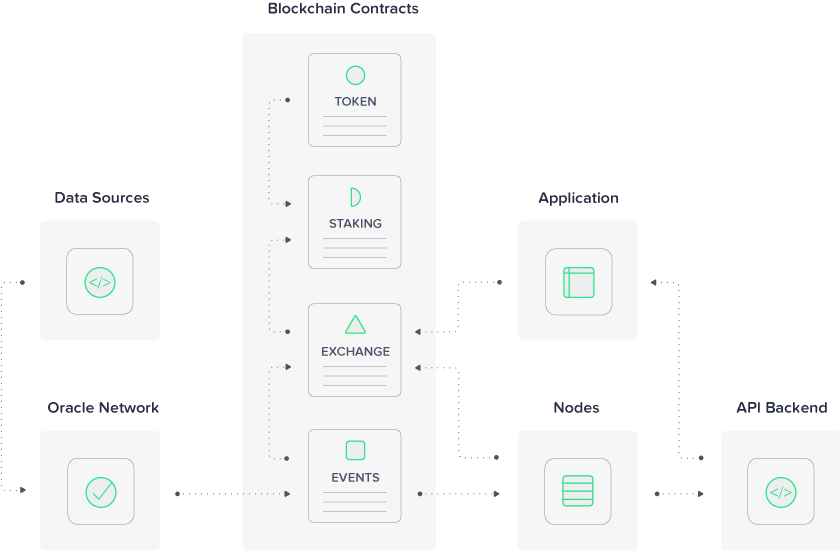
\includegraphics[scale=.35]{../Downloads/papers/architecture-diagram.png} 
\caption{Architectural overview of the platform infrastructure}
\label{figure:architecture}
\end{figure}


	\subsection{Exchange Layer}
	
The exchange layer refers to all blockchain infrastructure which facilitates critical exchange functionality. We use the term critical functionality to define any data or action which can directly influence the transfer of funds. Specific examples of this include:

\begin{itemize}
	\item Deposition, storage and withdrawal of funds
	\item Creation and storage of events
	\item Placement and cancellation of bets
	\item Bet matching
	\item Outcome resolution for bets (win, loss \& void)
	\item Staking and fee redistribution mechanisms
\end{itemize}

These functions are integral to the exchange and therefore require the security provided by blockchain technology. By leveraging the NEO platform, specifically smart contracts and nodes, we can provide the groundwork for a decentralized sports betting exchange.



		\subsubsection{Smart Contracts}
Smart contracts are programs used to read and write data to the blockchain. What makes these programs unique from an operational perspective are their immutability and decentralized execution. Once a contract is deployed it exists perpetually on the blockchain and is unable to be directly modified. Additionally, this program is not run by a single entity and is instead executed by all NEO nodes as they work towards block consensus. These properties mean that critical exchange infrastructure, such as fund transfers, bet placements and outcome decisions, can be made transparent, tamper free and independent of Block Sports.
 
Currently there are a number of contracts planned for initial release as detailed in Table \ref{table:contracts}. While we have done significant planning and testing which has lead to the development of prototypes, some aspects of these contracts are not yet finalized. 

\begin{table}[!htb]
\caption{Smart Contract Details}

\begin{tabularx}{\textwidth}{ p{3cm}  p{8.4cm}}
\bfseries{Contract} & \bfseries{Purpose} \\
\hline

Event & Used to access Event data stored on chain. \newline Facilitates oracles and the consensus of event creation and updates. \\   \hline

Exchange & Stores users funds and allows users to bet on events. \newline Interacts with the events contract allowing bets to be placed upon them. \\   \hline

Token & Maintains our NEP-5 compliant BSX token. \newline Facilitates the Block Sports ICO crowdsale. \\   \hline

Staking & Allows users to stake BSX tokens to retrieve \newline their share of fees generated by the exchange. \\

\hline

\end{tabularx}
\label{table:contracts}
\end{table}

		\subsubsection{Nodes}
Nodes are programs which sit outside of the blockchain and can be thought of as the link between the blockchain and non-blockchain programs. Their specific function is not predefined and instead is dependent on the use case of the platform. Seen in Table \ref{table:nodes}, Block Sports requires the use of a number of nodes to handle processing, event creation and data tracking. 

\begin{table}[!htb]
\caption{Node Details}

\begin{tabularx}{\textwidth}{ p{3cm}  p{8.4cm}}
\bfseries{Node} & \bfseries{Purpose} \\
\hline

Data & Observes the blockchain for updates to events and betting contracts. \newline Tracks all blockchain data changes and publishes this to the service layer. \\ 
\hline

Processing & Intelligently processes the matching queue. \newline Distributes winnings to users who have chosen the correct outcome. \\   \hline

Oracle & Run by trusted operators and used to relay event data to the blockchain. \\

\hline

\end{tabularx}
\label{table:nodes}
\end{table}

	\subsection{Service Layer}
Infrastructure which supports the user facing segment of the platform falls under the service layer category. The primary goal here is to provide infrastructure that enables a complex, feature rich product as opposed to an interface which presents itself as a developmental afterthought. Taking lead from a number of modern web applications, the architecture for the service layer utilizes ReactJS for all front-end interfaces and Go for its back-end server.  

		\subsubsection{Front-end}	
There is a relatively high level of sophistication required from the UI of a sports betting exchange. In comparison to traditional sports betting exchanges, this complexity is compounded due to the utilization of blockchain technology for matching, escrow and processing. Aspects such as wallet integration, blockchain processing and block time delays have the potential to create a confusing experience for platform users. Therefore, in alignment with the core objectives, the front-end has been designed to conceal this complexity and remain familiar and intuitive for both new and old exchange users. 

Upon release, the front-end will consist of a web application built with the ReactJS library. Aside from its performance strength and rising popularity, React can be used as both a mobile and desktop development library. This reduces the overhead required for the future mobile release while also paving the way for potential desktop clients.

		\subsubsection{Back-end}
What makes the Block Sports platform unique as a web application is that the core logic which typically constitutes as back-end is instead relegated to the blockchain layer. This reduces much  of the heavy lifting but introduces new responsibilities in order to act as an intermediary between blockchain data and the data seen by users. Some of these responsibilities include: 

\begin{itemize}
	\item Interacting with the data node to pull event and bet data
	\item Collating historical and account-specific data
	\item Organizing and serving data through the API
	\item Sending notifications for event and bet updates
\end{itemize}

Due to the direct communication made with exchange nodes, the decision for a back-end language was made between those directly supported by the NEO protocol. Outside of the direct plug and play capability, this helps maintain language uniformity throughout the platform. Go was chosen here due to its strong performance capabilities as both a server and a data processing language . 

\section{Blockchain Concepts}
	\subsection{Funds}
Users are enabled to use NeoGas (GAS) as the medium of exchange on the Block Sports platform. Since GAS is a global asset, a drawback is the inability to programmatically handle these assets within contracts. Without manual intervention as an option (as this suggests centralization), it is necessary to work around this limitation. 

The solution is to create a token equivalent to GAS (GASX) which is accredited to a user’s funds as a GAS deposit is made to the contract. By creating a NEP-5 token tethered to the value of GAS we can transfer GASX funds without the restrictions of a system asset. The consequence of this method is the two-step process required for a new user to place a bet on the platform - an initial step to deposit GAS and a second to place a bet with the newly acquired GASX. This solution means that users will have account funds separate from their wallet, requiring the explicit deposit and withdrawal of funds.

	
	\subsection{Events}
Events are the foundation of a sports betting exchange as their data is responsible for triggering and validating processing across the platform. Users must therefore trust this data completely as its inaccuracy could lead to the incorrect loss of funds. This importance was the catalyst for the implementation of an oracle network which ensures majority consensus on event data before it it is published to the blockchain.

The lifecycle of an event is as followed:
\begin{enumerate}
	\item Oracle A discovers a new event and publishes it to the blockchain
	\item An unvalidated event is created and stored against a generated event ID
	\item Oracle B discovers the same event, publishes and increments this discovery
	\item Repeat until majority consensus is reached, triggering event validation and enabling bets
	\item Bets are permitted against the event until 10 minutes before commencement
	\item Event finishes, Oracle X fetches and publishes results to the blockchain
	\item Oracle Y fetches the same results, publishes and increments this outcome
	\item Repeat until a majority consensus is reached, triggering outcome validation and enabling fund collection
	\item \it{If a consensus is not reached, the event is voided and all funds are redistributed}
\end{enumerate}

		\subsubsection{Event Structure}
When an oracle publishes an event it must send through the data fields seen in Table \ref{table:events}. Given that the initial release will focus on head to head matchups the structure is kept minimal and requires only the fields which can uniquely identify the event. While most of the information is stored as serialized data for improved performance, the start date and draw flag are stored individually to be used in the validation process of bet placements. 

\begin{table}[!htb]
\centering
\caption{Event Object}

\begin{tabular}{ c c }
\bfseries{Field} & \bfseries{Description} \\
\hline

name & Event Name \\ 
\hline
sport & Event Sport \\  
\hline
competition & Event Competition \\ 
\hline
home & Home Team \\ 
\hline
away & Away Team \\ 
\hline
start & Start Date (UNIX Time) \\ 
\hline
draw & Can Draw (True/False) \\ 
\hline

\end{tabular}
\label{table:events}
\end{table}

		\subsubsection{Event Creation}
When an oracle discovers a new event via their source this data is published to the event contract for on-chain consensus. To perform consensus, the contract generates an Event ID and checks whether other oracles have done the same. If majority consensus is met the event becomes validated for bets to be placed on its outcome.

			\myparagraph{ID Generation}
Event IDs are created by performing a hash on the the serialized event fields in the form seen below. This provides us with a unique identifier of a fixed 24 character length, making it easier to reference and store data against this ID. 


\begin{center}
name-sport-competition-home-away-commence-draw
\end{center}
	
		\subsubsection{Updating Events}
There are two scenarios in which an event can be updated - when an outcome has been decided or when the event has been voided (See Section 5.8). Similar to the creation of an event, an update is validated after on-chain consensus has been reached by the oracle network. After this validation occurs users are enabled to collect either their winnings or their voided/ unmatched funds.  

	\subsection{Bets}
	After the validation of an event by our oracle network, permission is given to users to place bets on an outcome. Performing this action requires an invocation to the betting contract, an operation which can be executed both manually or through our web application. The successful placement of a bet results in a new, unmatched bet being stored on the blockchain as it waits to become matched by another user.
	
		\subsubsection{New Bet Structure}
When placing a new bet there are five fields which are required for successful placement. This is shown in Table \ref{table:bets}.

\begin{table}[!htb]
\centering
\caption{New Bet Object}

\begin{tabular}{ c c }
\bfseries{Field} & \bfseries{Description} \\
\hline

eventID & ID of the Event \\ 
\hline
outcome & Chosen Outcome \\  
\hline
odds & Chosen Odds \\ 
\hline
type & Type of Bet (Back or Lay) \\ 
\hline
amount & Amount to Place on Bet \\ 
\hline

\end{tabular}
\label{table:bets}
\end{table}

	\subsubsection{Validation}
Bet validation is essential in order to prevent users from placing erroneous or malicious bets on the exchange. Key validation includes confirming the validity of an event, the existence of an outcome and that the user possesses funds greater than the bet amount stipulated. 

\subsubsection{Cancellation}	
Bet cancellation is possible on the condition that the bet has remained entirely or partially unmatched. As the economy of the exchange is dependent on its equilibrium, cancelling a matched bet would require the restoration of funds which have been pre-allocated to another user. If the conditions have been met, a bet can be cancelled by simply calling the contract with the desired bet to cancel, at which point funds will be returned given a small cancellation fee. 

	\subsection{Matching}
The mechanism for matching bets can be seen as the limiting factor for decentralized exchanges as its performance dictates the volume your platform can operate at. Solutions put forth by currency exchanges, hybrid or otherwise, typically involve an off-chain matching engine which is run by a single entity. By placing order matching off-chain, an exchange’s matching performance is suddenly unrestricted from on-chain limitations. The caveat is that off-chain matching requires a single authority to enforce these matches on-chain, going against the principles of decentralization. 

The situation faced by Block Sports is that we require our exchange framework to remain functional without the necessity for a central authority. This rules out the possibility of an off-chain system without going to lengths to create and ensure the decentralization of this aspect. What we therefore propose is a novel take on the matching engine, removing the need for a central authority by placing bet matching on-chain and allowing it to be executed by any user. While there will be a trade-off in performance, this method ensures the platform can continue to operate in the unlikely scenario Block Sports goes offline. In this scenario, the worst case for the user is not a loss of funds, just downtime before they can retrieve their funds again. 	

\subsubsection{Matching Procedure}
When a bet is placed it is stored at the end of the queue for its specific market. This market is defined by the Event ID, Odds and Outcome it was placed upon. In order for a bet to become matched there must be a bet of the opposite type within this market, e.g. a ‘back’ bet requires a an opposing ‘lay’ bet within the same market and vice versa. These ‘back’ and ‘lay’ bets are referred to as partners or pairs. The matching process itself involves specifying a market and matching its queue with its opposing partner queue until either has been exhausted or the GAS consumption limits are reached. 

The implication of giving control to the user to process bet matching is that it can be abused. However this processing operation means bets are matched on a first in first out basis within a market, preventing users from prioritising their own bets. There is opportunity for users to prioritise their own market to complete its matching though this will not block other markets from being matched. While anyone can process these queues there is no expectation on the user to do so given Block Sports is operational. What will be provided is a node whose job is to optimally execute this function and match on behalf of users. 


	\subsection{Distributing Winnings}
Winnings can be collected after an event’s outcome has been validated. Due to the nature of the Neo blockchain, it is infeasible for the distribution of funds to occur as an on-chain response to an event’s outcome. A solution to this is to employ a collection mechanism used to distribute winnings to those which have selected the correct outcome or are owed the return of funds.

Similar to the mechanism employed by matching bets, the ability to distribute winnings does not require permissions to perform. This is possible as winnings are credited towards the bet maker as opposed to the contract invoker. Although it initially makes sense to restrict the collection of winnings to the user which performed the bet, by removing restrictions it becomes possible to distribute funds to a user on their behalf. As a result of this, Block Sports is able to provide a node which distributes winnings to users without their action, with the fallback of self-collection if required.
		
		\subsubsection{Void Events}
Given the situation in which an event is made void, all bets made within this event are immediately voided and are able to be retrieved through the normal fund distribution method. This is an unlikely scenario however and occurs for reasons such as disqualifications, event delays or postponement.

		\subsubsection{Oracle Reliance}
In the event the oracle network does not come to a consensus on an outcome, the match is considered voided after a certain period of inactivity, allowing users to retrieve their funds for that event. This guarantees that funds are unable to be locked within the contract, ensuring that the worst case scenario is not a loss of user funds, but instead just a loss of opportunity.


	\subsection{Fee Distribution}
There are two categories of Block Sports users which are eligible to receive a share of generated platform fees - BSX token holders and oracle operators. These users are allotted an apportioned amount of fees and are able to claim these fees periodically via invocation of the staking contract. 

		\subsubsection{Token Holders}
Token holders are eligible for fee distribution as part of a dividends system, helping link the value of the BSX token to the volume of the exchange. When a user stakes their token they elect a period of time for their token to be held by the staking contract. During the time of their nominated period a user may regularly collect their allocated fees while their tokens are held. The longer a user chooses to stake their tokens, the greater a fee proportion is given to that user. Equation \ref{eq:token-dist} details the token holder fee distribution:

\begin{equation}
F = R\times A\times S/T\label{eq:token-dist}
\end{equation}

Where F is the given share of fees, R is the fee proportion rate based on staking period, A is the funds available for distribution, S is the staked amount of tokens and T is the total supply of tokens.

		\subsubsection{Oracle Operators}
Oracle operators claim fees in a similar manner to token holders without the constraint of token staking. Instead, when an oracle is newly whitelisted they are registered to the staking contract and allowed to claim funds periodically during their activation. If an oracle is subsequently blacklisted they are removed from this contract and are unable to continue their claims after this point. The simpler dynamic of this fee distribution requires a simpler calculation, as shown in Equation \ref{eq:oracle-dist}:

\begin{equation}
F = A\times 1/N\label{eq:oracle-dist}
\end{equation}

Where F is the given share of fees, A is the funds available for distribution and N is the total number of non Block Sports oracles.

\section{Oracles}
An oracle acts as a bridge between off-chain data and on-chain contracts, working to validate and subsequently publish this external data to the blockchain. Due to the inability for smart contracts to query outside of the blockchain network, a common workflow involves using an oracle as a proxy, observing the blockchain for query ‘requests’, retrieving and validating the desired data and finally publishing this data to the requesting contract. 

Given that Block Sports stores events and bets on-chain there is no requisite for contracts to initiate off-chain queries as other Dapps might - a characteristic which significantly improves the user betting workflow. Instead, we use oracles to publish trusted event fixtures and updates to the blockchain before bets can be placed or won on their outcome. By doing this we move the time and complexity of data validation to a phase which does not impact the end user. 

The following features are an outline of the primary functions of a Block Sports Oracle:

\begin{itemize}
	\item Regularly fetch event data from an external source
	\item Standardise data to fit Block Sports specifications
	\item Publish new events and outcomes to the blockchain
	\item Observe the blockchain for updates made by other oracles
\end{itemize}

	\subsection{Decentralization}
	It is important to eliminate the risk of erroneous or malicious data being published to the blockchain. If users are unable to trust the data used to dictate events and outcomes, they will be less inclined to entrust their funds to the platform. While running a single self-controlled oracle node to publish data is passable as a solution (and similar to the solutions employed by centralized services), we see it as contradictory to the underlying principles of the platform - security and decentralization. 

There are two measures we can take to alleviate the risk of a single entity having too much authority over published data. Firstly, we can distribute the responsibility of publishing data across many oracles, both self-run and externally operated, and necessitating majority consensus on data before it is validated and usable. Secondly, we can stipulate the use of multiple data sources across these oracles. 

		\subsubsection{Consensus}
The proposal is for an on-chain consensus mechanism in which trusted oracles vote by publishing data they believe to be true. When a majority of oracles have published the same data, either an event fixture or outcome, the blockchain will accept this data as verified and enable access for the betting contract. A basic version of this concept can be seen in our prototype contract. Opting for on-chain consensus allows us to reduce the oracle network complexity by utilising the security and immutability native to the NEO blockchain. This helps further ensure user trust in the platform and in the security of their funds. 

		\subsubsection{Data Sources}
Data sources are external to the Block Sports platform and provide oracles with the event data they publish to the blockchain. Each oracle designates a single source as their data feed, with the intention of employing many unique sources across all operating oracles. Utilizing multiple sources has obvious benefits to the integrity of the data published - if multiple oracles are reaching consensus on multiple datasets we have greater confidence in its accuracy. This also addresses the original concern of centralization by eliminating another single point of failure in the data pipeline. 

	\subsection{Operation}
As distribution of authority is a requirement for decentralization, partnering with third party oracle operators is necessary. The ability to operate an oracle will be open to any member of the Block Sports community, with limited positions opening up as the platform progresses its rollout. These limitations exist to maintain quality control across oracles and to sustain financial incentivization. Early stage operators will be hand selected community members while later stage operators will be voted in or transferred with existing spots. By operating an oracle you are entitled to a percentage of the platform fees which are then equally distributed amongst all non Block Sports operators.

The oracle code itself will be open sourced with guidelines on setup, operation and associated costs. The intention is to decrease the bias towards developers by reducing the barrier of entry and allowing non-technical investors to participate. Most operators will have the choice over the data source they choose to use and how this is standardised to Block Sports format. This relies on coding, therefore if an operator wishes to use an API which has not been used by other oracles there will be development guidance from Block Sports. In practice a data source will not be restricted to a single oracle however there will be strict limitations on the number of simultaneous connections. Possible choices for a source include paid APIs or custom built web scrapers. Manual entry may also be initially viable, however when the exchange scales up in both events and markets, this method becomes unreliable leading to the oracle not meeting the standards of operation. 

	\subsection{Oracle Rollout}
The oracle network will be rolled out in four stages. By incrementally releasing we are able to deliver our product to market sooner, allowing analysis and refinement as the platform scales larger. Each stage represents greater decentralization and will release corresponding to platform growth as a means to improve security as volume (risk) increases. The rollout takes the platform from a small network operated internally by Block Sports to an entirely decentralized and autonomous oracle network ecosystem. 

		\subsubsection{Stage One}
		The initial MVP release of the oracle network will consist of a small number of oracle nodes utilizing a single high quality data source. These nodes will be solely operated by Block Sports, making the in-house nature of this stage analogous to more centralized sports betting services. This stage can be thought of as a beta for the oracle network and will allow close supervision over the network as the platform is first released. The plans are to maintain this stage until we reach an exchange throughput which both validates the platform and properly incentivizes the progression to stage two.
		
		\subsubsection{Stage Two}
		As the platform gains volume and is identifiably stabie we will move into stage two of the oracle rollout. This involves the transfer of ownership of a majority of Block Sports oracles to external, trusted parties in the community such as established partners and community groups. To help foster growth, Block Sports will cover any costs associated with data sources at this stage. This will offset the low initial exchange volume and attract greater interest by allowing operators to receive the full benefit of operation. At this stage automatic fee claiming will be available, however permission and access management for oracle nodes will be manually managed by Block Sports [see section 8.1 for more information on fee claiming].

		\subsubsection{Stage Three}
		Until stage three, the sources across all oracles will have been limited to a single trusted third party feed. As the platform reaches higher volume and greater security is required we will both increase the number of oracles and enforce data source diversity across the network. At this point, costs will become the responsibility of operators as they are encouraged to pursue alternative sources. There will be a direct effort by Block Sports to help this transition by monitoring alternatives and contributing to the development of scrapers or potential crowd sourcing solutions.
		
		\subsubsection{Stage Four}
		When the platform has matured and gained more mainstream traction, resources will be focused towards developing an autonomous oracle ecosystem. This means removing any required oversight Block Sports has over the network, namely oracle monitoring, blacklisting and whitelisting. Stage four is therefore the implementation of this solution. This stage comes at a phase much later than the established company roadmap and as such, solutions are not finalized. However it is important to indicate our intention to reach this stage and we will release further information to the public as it is available.
		
\section{Company}
	\subsection{Roadmap}
	
\begin{itemize}
   
   \item 2018 Q1 [Delivered]
   \begin{itemize}
     \item Smart Contract Prototypes
     	\begin{itemize}
     		\item Proof of concept smart contracts, designed to show off core sports betting functionality. Publicly available on our github.
     	\end{itemize}
   \end{itemize}

   \item 2018 Q2 [Delivered]
   \begin{itemize}
     \item Functional Exchange Demo
     	\begin{itemize}
     		\item Proof of concept exchange demo for demonstrating the vision for the platform. Publicly available on our website.
     	\end{itemize}
   \end{itemize} 

   \item 2018 Q3
   \begin{itemize}
     \item Crowdsale
     	\begin{itemize}
     		\item ICO Crowdsale to help raise operational funds. Details will be announced as soon as technical and legal preparations are complete
     	\end{itemize}
     \item Hiring
     	\begin{itemize}
     		\item Several roles ranging from development to design will be filled for the first 12 months of development
     	\end{itemize}
      \item Exchange Listing
     	\begin{itemize}
     		\item Listing of BSX tokens on exchanges. This is expected to happen within 30 days of the crowd sale. There will be discussion with exchanges prior to the token sale, with more clarity being provided closer to this date
     	\end{itemize}
   \end{itemize} 
   
   \item 2019 Q1
   \begin{itemize}
     \item TestNet Beta
     	\begin{itemize}
     		\item Functional smart contracts will be made publicly available on the Neo TestNet. These contracts will be a finalized version of the prototypes with full functionality and interface for input/output
     	\end{itemize}
     \item Oracles
     	\begin{itemize}
     		\item Stage one of the oracle network will be launched for smart contract integration and testing
     	\end{itemize}
   \end{itemize}    
 
    \item 2019 Q2
   \begin{itemize}
     \item Exchange Beta
     	\begin{itemize}
     		\item Fully functional service and exchange layers operating on the Neo TestNet. Upon this release, user testing and security auditing will be the primary focus 
     	\end{itemize}
   \end{itemize} 
   
   \item 2019 Q3
   \begin{itemize}
     \item Full Exchange Release
     	\begin{itemize}
     		\item Full release of the Block Sports Exchange on the Neo MainNet
     	\end{itemize}
   \end{itemize} 
   
\end{itemize}

Note: There are many other plans for the future of Block Sports which we will detail at a future date. This roadmap lists the core items we are confident in committing to at this stage. 

	\subsection{Legal Structure}
Block Sports is limited liability company registered in Macedonia (FYROM). We are compliant with all gaming, financial and securities laws relevant to our platform within the laws and regulations of Macedonia (FYROM).
	
	\subsection{Auditing}
Third party auditing services will be engaged throughout the development process to ensure that all aspects of the Block Sports Exchange are secure. As well as professional auditing, 
bug bounty programs will be launched alongside the Exchange Beta release. 
	
\section{BSX Token}

Unlike many platform projects, the BSX token is not a utility token used for betting. BSX is a dividend bearing token, providing holders a share in platform fees. The more volume bet on the Block Sports Exchange the more fees that are generated in turn increasing the value of the token. This model ensures token value is directly tied to the success of the platform. 

	\subsection{Platform Fees}
Upon the completion of a successful bet a 2\% operational fee is charged from the winnings and the remaining 98\% is credited to the winner. Fees are then accumulated in a pool and then redistributed at the following rates:

\begin{itemize}
	\item 75\% to the holders of staked BSX *
	\item 5\% to active oracle operators **
	\item 20\% to the Block Sports company in order to fund development long term

\end{itemize}

* Users staking BSX tokens are entitled to a share of fees proportionate to the total supply of BSX tokens. 

** Active oracle operators will receive an even share in BSX tokens proportionate to the total number of oracles. For example if there were 20 oracles, each oracle would be entitled to 1/20 or 5\% of the oracle operator fee distribution.

\section{Token Sale}
The Block Sports public token sale will be held during the third quarter of 2018, the exact date has not yet been decided as important prerequisites are yet to be finalised. Specific token sale details such as price, supply, distribution and timelines are not yet finalised. When this information is available, this document will be updated.

	\subsection{KYC Requirements}
Terms and conditions for the crowdsale are not yet finalized. Whitelisting will be required for participation in the Block Sports token sale.

	\subsection{Individual Investor Cap}
The individual investment cap for each participant will be determined no less than 24 hours prior to the beginning of the token sale. 
	
	\subsection{BSX Token Distribution}
A visual breakdown of the BSX token distribution is shown below in Figure \ref{figure:distribution}. During the public crowdsale 70\% of the total BSX tokens will be available to investors. 19\% of the remaining tokens will be held in operational reserve, 10\% will be allocated to the team and 1\% will be immediately unlocked and distributed within 6 months to early contributors and partners. T

\begin{figure}[!htb]
\centering
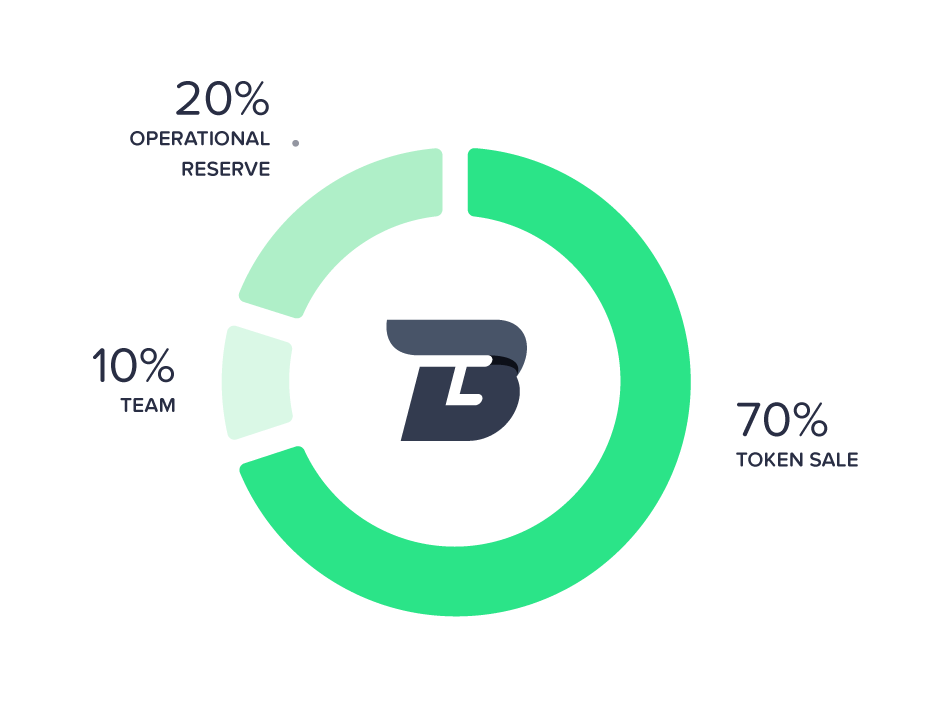
\includegraphics[scale=.2]{../Downloads/papers/tokensale-diagram.png} 
\caption{BSX Token distribution}
\label{figure:distribution}
\end{figure}

	\subsection{Vesting}
To ensure alignment to the success of the project, tokens reserved for the Block Sports company and founders will be vested for a period of 18 months with a 12 month cliff. After the 12 month cliff, vested tokens will be released in equal portions on a quarterly basis. All tokens will be released 18 months after the completion of the crowdsale. 

\begin{figure}[!htb]
\centering
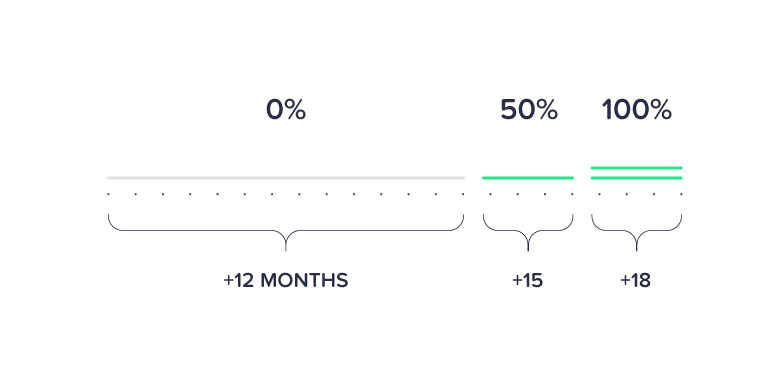
\includegraphics[scale=.3]{../Downloads/papers/vesting-diagram.png} 
\caption{Visual breakdown of employee vesting}
\label{figure:vesting}
\end{figure}
	

	\subsection{Fund Allocation}
The primary focus in the first year of operation is releasing a product to the market. With this in mind resources are focused on development.

Projected use of company funds in the first year of operations:

\begin{itemize}
	\item  65\% Product \& Development (Blockchain development, product design, product development, sports data)
	\item 15\% Operational (Utilities, administration, technology, tools and general expenses)
	\item 10\% Marketing and outreach (marketing materials, events, staff and services)
	\item 10\% Legal and Accounting
\end{itemize}

Upon the release of the Block Sports Exchange, more resources will be focused on marketing, with a focus on user growth

Projected use of company funds in the second year of operations: 

\begin{itemize}
	\item 40\% Product \& Development (Blockchain development, product design, product development, sports data)
	\item 35\% Marketing and outreach (Advertising, marketing materials, events, staff and services)
	\item 15\% Operational (Utilities, administration, technology, tools and general expenses)
	\item 10\% Legal and Accounting
\end{itemize}

\end{document}
